\section{IT Service Level Management}

\subsection{Sie kennen das IT Service Level Management und können einen IT-Service und ein Service Level Agreement erläutern.}
Bildet die Schnittstelle zwischen Service Provider und Kunde und trägt so dazu bei, dass die Anforderungen des Kunden erfasst, dokumentiert und schliesslich bei der Gestaltung des Services umgesetzt sowie die SLA-konforme Erbringung der Services dem Kunden nachgewiesen wird. Leistet einen wichtigen Beitrag zur Entwicklung der Beziehung zwischen Kunde und Service Provider.

Das Service Level Managment stellt sicher, dass IT Services auf einem geforderten und akzeptablen Mass erbracht werden. Das bedeutet, dass die Anforderungen verstanden worden sind und eine Vereinbarung über die zu erwartende Qualität getroffen wurde.

Wir unterscheiden unterschiedliche IT Service Vereinbarungen (siehe Abbildung \ref{fig:it-service-mgmt-service-vereinbarungen}):

\begin{itemize}
	\item \textbf{SLA} Service Level Agreement: Vereinbarung zwischen Service Provider und Kunde bezüglich Qualität und Quantität sowie der Ziele für die Service-Erbringung.
	\item \textbf{OLA} Opertional Level Agreement: Das sind interne Vereinbarungen zwischen unterschiedlichen Organisationsstrukturen. Und dienen als Absicherungen für einen übergeordneten SLA. Diese sind nicht juristisch bindend.
	\item \textbf{UC} Underpinning Contract: Das ist im Prinzip die formale Variante der internen OLA für Vereinbarungen mit externen Partnern. Hier werden alle Leistungen festgehalten, welche nicht vom Service Provider selber erbracht werden oder sollen.
	\item \textbf{SLR} Auf der Folie steht die Abkürzung SLR für Service Level Request. Das ist falsch. Es steht für Service Level Requirement. Hier werden nämlich die Anforderungen des Kunden dokumentiert und dienen als Basis für die SLAs.
\end{itemize}

\begin{figure}[h!]
\centering
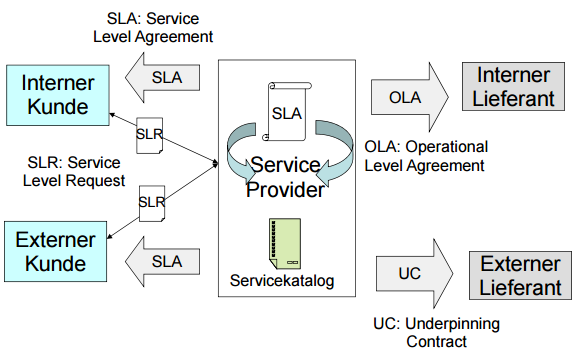
\includegraphics[width=0.7\linewidth]{fig/it-service-mgmt-service-vereinbarungen}
\caption{Service Vereinbarungen}
\label{fig:it-service-mgmt-service-vereinbarungen}
\end{figure}

\subsubsection{SLA}
Das Service Level Agreement besteht aus einer Servicebeschreibung, einem Betriebsfenster und einer bestimmten Verfügbarkeit. Ausserdem soll irgendeiner Form die Performance beschrieben werden. Zudem muss auch RPO (Recovery Point Objective, Datenverfügbarkeit, Welcher Datenzeitpunkt nach Recovery?) und RTO (Recovery Time Objective, Wiederherstellungszeit, Wie Lange?) beschrieben werden nach einem Desaster.
Zudem muss zu jedem SLA definiert werden, welche OLAs zugrunde liegen. Diese Dienstleistungen kauft der Service Provider auch selber ein. Schlussendlich muss dokumentiert sein wie hoch der Preis ist (Pauschale, Flatrate, Pro Benutzer, pro Anfrage, pro Transaktion).
SLAs müssen überwacht und regelmässig den Benutzer rapportiert werden. Bei starken Abweichungen vom SLA-Vertrag müssen Massnahmen für Verbesserungen eingeleitet werden.

Man sollte nicht wahllos mit Betriebsfenster und Verfügbarkeiten spielen. 24 * 7 Betriebsfenster sind extrem teuer auch eine Verfügbarkeit von 99.999 Prozent ist extrem teuer.

\begin{figure}[h!]
\centering
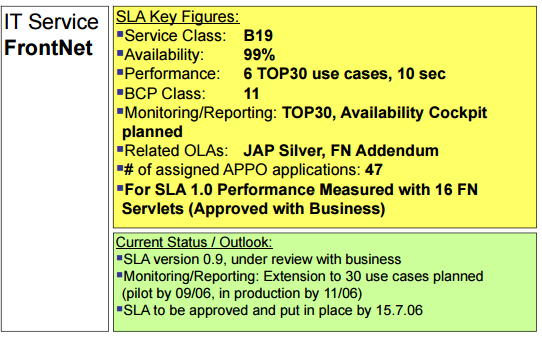
\includegraphics[width=0.7\linewidth]{fig/beispiel-sla}
\caption{Beispiel SLA Beschreibung}
\label{fig:beispiel-sla}
\end{figure}

\begin{figure}[h!]
\centering
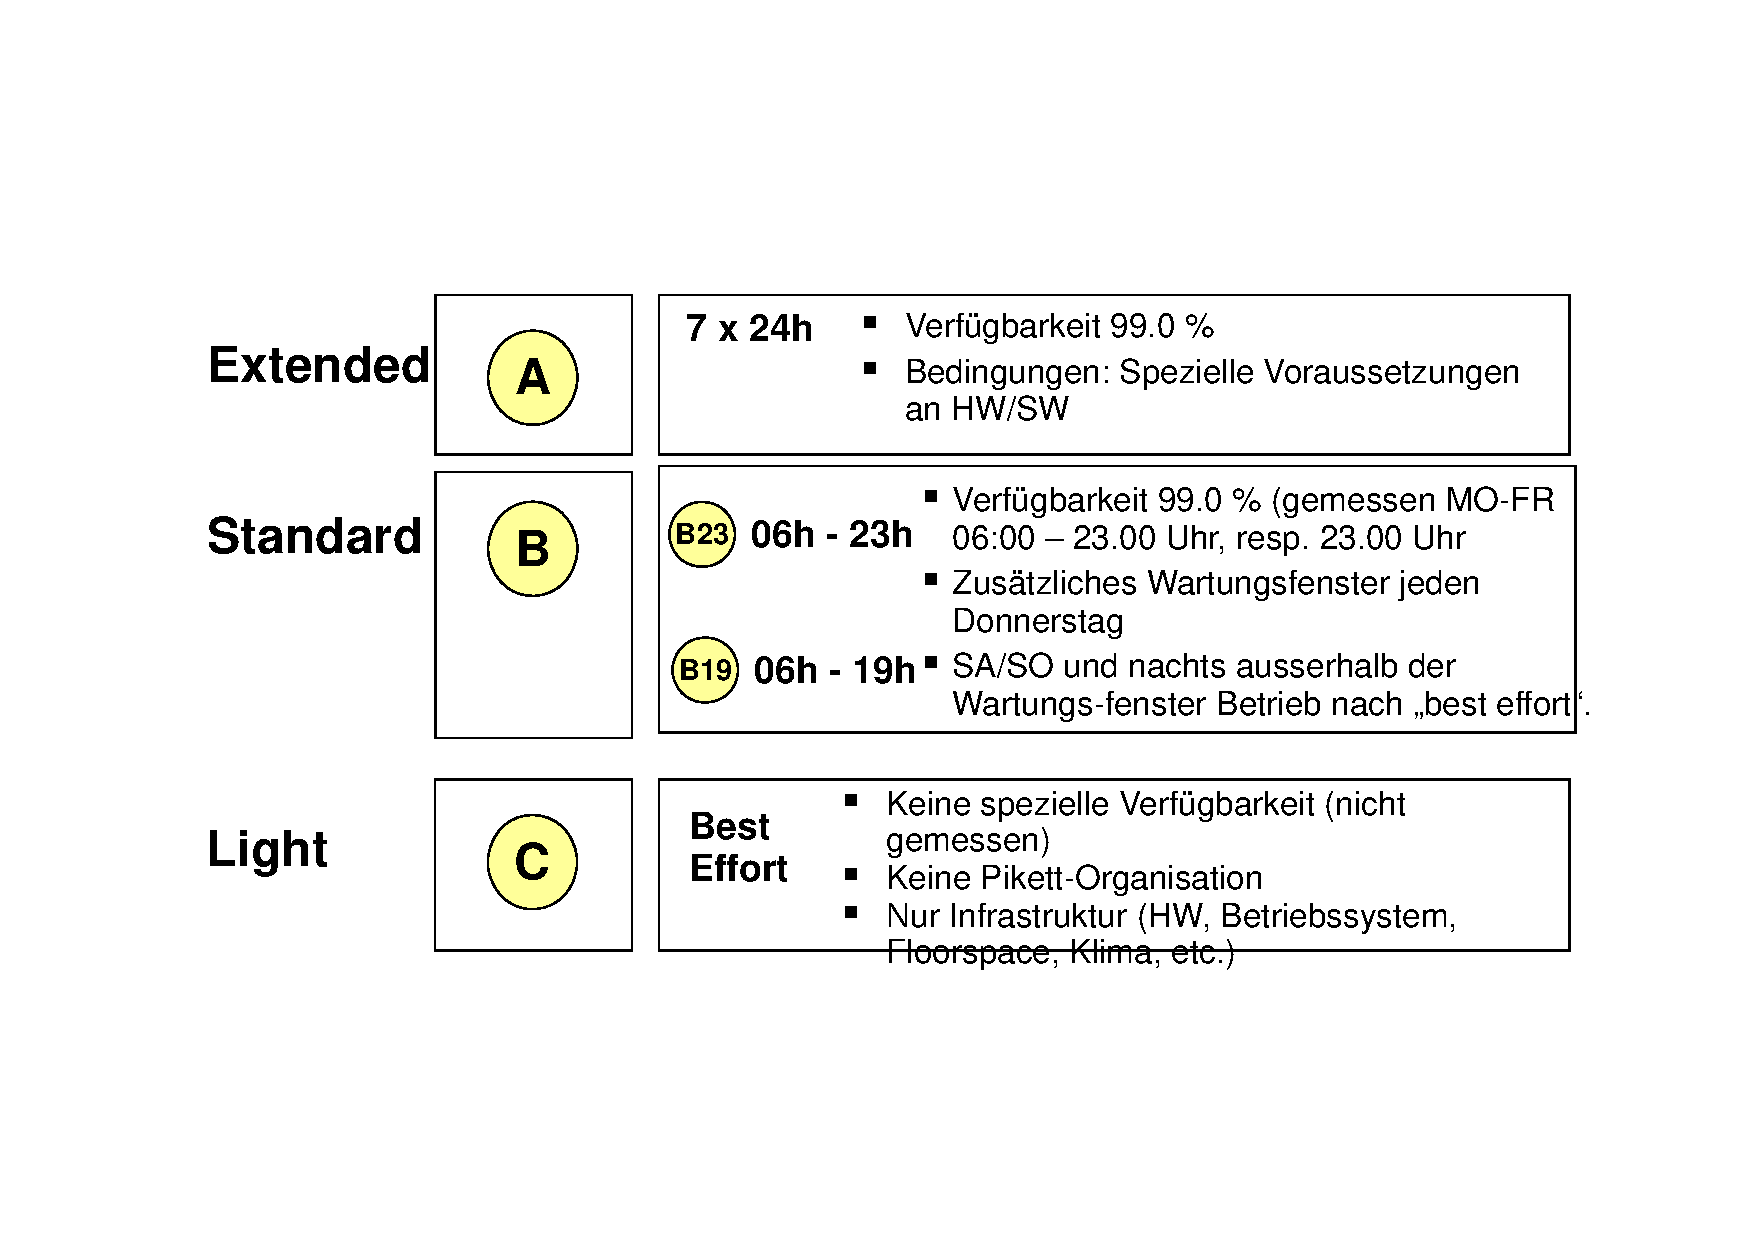
\includegraphics[width=0.7\linewidth]{fig/beispiel-schlaue-sla-klassen}
\caption{Beispiel gescheite SLA Klassen}
\label{fig:beispiel-schlaue-sla-klassen}
\end{figure}

\subsection{Sie können einen Service Level Katalog erstellen und sind in der Lage einen IT-Service zu beschreiben.}

Ein möglicher Service Katalog ist auf Abbildung \ref{fig:beispiel-service-katalog} dargestellt.

\begin{figure}[h!]
\centering
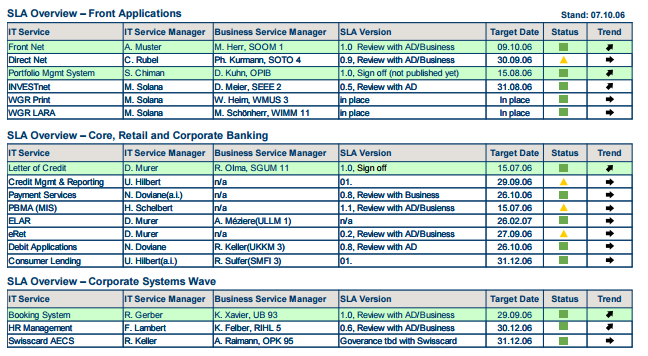
\includegraphics[width=0.7\linewidth]{fig/beispiel-service-katalog}
\caption{Beispiel Service Katalog einer Bank}
\label{fig:beispiel-service-katalog}
\end{figure}

\subsection{Sie können die Budgetierung der Kosten für ein Betriebsteam oder für einen kleinen Servicedienstleister durchführen.}

Ein Budget wird für die Periode EINES Jahres erstellt. Das heisst, alle Kosten und Einnahmen werden auf ein Jahr runtergebrochen. Man unterscheidet zwei Kostenarten: Laufende Kosten (Löhne, Miete) werden direkt in eine Jahresbudget eingerechnet. Investitionskosten (Kaufkosten für einen Server) werden über Abschreibungen in ein Jahresbudget verrechnet. Abschreibungen in der IT werden linear auf 3 bis 5 Jahre durchgeführt. Zu einem Budget gehören auch die Einnahmen respektive die Verteilung der Kosten auf die Services.

Um nun ein Budget zu erstellen sind zusätzliche Angaben notwendig: Mietkosten, Personalkosten, Infrastrukturkosten (Hardware, Software).